\section{Nonlinear acoustics and derivative nonlinearities}
\label{acou:sec}

High-intensity ultrasound (HIFU tissue ablation, shock-wave lithotripsy,
ultrasonic cleaning and welding) and sonic-boom propagation are described, to
second order in the acoustic Mach number, by the Westervelt and Kuznetsov
equations \cite{HamiltonBlackstock1998,Kaltenbacher2015}. Their
nonlinearities are quadratic in \emph{derivatives} of the unknown and they are
quasilinear. We ask which of these models, and two semilinear caricatures,
show ODE-type self-similar blowup, and how far the method of \cref{fw:sec}
carries. As in \cref{geom:sec} we mark statements as
\textbf{(K)} known (with reference), \textbf{(D)} derived or proved here
(proof or proof sketch given, formulas checked in
\texttt{code/acou\_symbolic.py}), \textbf{(C)} conjectural, formal or
numerical only.

\subsection{Models}
\label{acou:sub-models}
\textbf{(K)} With acoustic pressure $p$, velocity potential $\psi$, ambient
density $\rho_0$, sound speed $c$, coefficient of nonlinearity
$\beta=1+B/(2A)$ and diffusivity of sound $b$, the Westervelt equation in
pressure form reads
\begin{equation}\label{acou:west}
  (1-2kp)\,p_{tt}-c^2\Delta p-b\Delta p_t=2k\,(p_t)^2,\qquad
  k=\frac{\beta}{\rho_0c^2},
\end{equation}
i.e.\ $p_{tt}-c^2\Delta p-b\Delta p_t=k(p^2)_{tt}$. It is obtained by
applying $\partial_t$ to the potential form
$\psi_{tt}-c^2\Delta\psi-b\Delta\psi_t=\beta c^{-2}\partial_t(\psi_t^2)$ and
setting $p=\rho_0\psi_t$. The Kuznetsov equation is
\begin{equation}\label{acou:kuz}
  \psi_{tt}-c^2\Delta\psi-b\Delta\psi_t
  =\partial_t\big(K\psi_t^2+|\nabla\psi|^2\big),\qquad K=\frac{B}{2A}\,c^{-2}
\end{equation}
\cite{Kuznetsov1971,Westervelt1963,Kaltenbacher2015}.
% TODO verify: bibliographic data of Kuznetsov1971, Westervelt1963, HamiltonBlackstock1998 (bib/acou.bib, from memory)
\textbf{(D)} The two
right-hand sides differ exactly by
$\partial_t\big(|\nabla\psi|^2-c^{-2}\psi_t^2\big)$, the time derivative of
the (negative) \emph{null form} $Q_0(\psi,\psi)$: the classical argument that
``local nonlinear effects'' are negligible for progressive waves is the
statement that $Q_0$ vanishes on plane waves.

\emph{Nondimensionalisation.} With $u=2kp$, $t\mapsto t_0t$, $x\mapsto ct_0x$,
\eqref{acou:west} becomes
\begin{equation}\label{acou:west-nd}
  (1-u)\,u_{tt}-\Delta u-\varepsilon\Delta u_t=(u_t)^2,\qquad
  \varepsilon=\frac{b}{c^2t_0}.
\end{equation}
For water ($\rho_0c^2\approx2.2\,$GPa, $\beta\approx3.5$,
$b\approx4\times10^{-6}\,\mathrm{m^2/s}$; standard handbook values, cf.\
\cite{HamiltonBlackstock1998}) the degeneracy $u=1$ corresponds to
$p^\ast=\rho_0c^2/(2\beta)\approx 3\times10^{2}\,$MPa, and the viscous time
scale is $b/c^2\approx2\times10^{-12}\,$s.

\emph{Two semilinear caricatures.} Freezing the coefficient $1-u$ to $1$ and
setting $\varepsilon=0$ in \eqref{acou:west-nd} gives the \emph{Riccati wave
equation}; replacing $(u_t)^2$ by the null form gives Nirenberg's example:
\begin{equation}\label{acou:models}
  \text{(RW)}\quad u_{tt}-\Delta u=(u_t)^2,\qquad\qquad
  \text{(NF)}\quad u_{tt}-\Delta u=(u_t)^2-|\nabla u|^2 .
\end{equation}
(RW) keeps the ``cumulative'' part $2kp_t^2$ of $k(p^2)_{tt}=2kpp_{tt}+2kp_t^2$
and drops the quasilinear part; (NF) is the semilinear analogue of the local
nonlinear effects.

\subsection{Shocks versus ODE-type blowup}
\label{acou:sub-which}
\textbf{(K)} For propagating waves the generic singularity is a shock: in
1D, simple waves of \eqref{acou:west} obey Burgers' equation and steepen at
the shock-formation distance while $p$ stays bounded
\cite{HamiltonBlackstock1998}; in several dimensions shock formation for
quasilinear wave equations is a different, geometric theory
\cite{Christodoulou2007}. % TODO verify bib data of Christodoulou2007 (from memory)
Shocks are not ODE-type blowup and lie outside the
semigroup method. ODE-type blowup instead requires a spatially
\emph{coherent} drive (in phase over a region larger than $c(T-t)$), such as
a uniform compression. \textbf{(D)} The spatially homogeneous dynamics are:
\begin{itemize}[nosep]
\item (RW), (NF): $u_T(t)=-\log(T-t)+c_0$ (exact), so that $u$ and $u_t$ blow up.
\item Westervelt, $b=0$: with $q:=1-2kp$, \eqref{acou:west} is equivalent to
  \begin{equation}\label{acou:qeq}
    (q^2)_{tt}=2c^2\Delta q .
  \end{equation}
  Homogeneous solutions have $q^2=A(T-t)$ (plus a constant), so
  $p\to1/(2k)$ stays bounded while $p_t=\sqrt A/(4k\sqrt{T-t})$. This is a
  \emph{degeneration}, not a blowup of $p$: the coefficient of $p_{tt}$
  vanishes and the local sound speed $c/\sqrt q$ becomes infinite.
\item Kuznetsov, $b=0$: $\psi=\psi(t)$ forces $(1-2K\psi_t)\psi_{tt}=0$, so
  there is \emph{no} homogeneous blowup, Riccati-type or otherwise (the
  right-hand side of \eqref{acou:kuz} is a total time derivative). The
  uniform compression $\psi=f(t)+B_0|x|^2/(2dc^2)$, whose velocity field is
  linear in $x$, solves \eqref{acou:kuz} if and only if
  $(f'-Kf'^2)'=B_0$, and it reaches the same degeneracy $\psi_t\to1/(2K)$
  with $\psi_{tt}\sim(T-t)^{-1/2}$.
\end{itemize}
The remaining subsections treat (RW) (\cref{acou:sub-rw,acou:sub-spec,acou:sub-nonlin}),
(NF) (\cref{acou:sub-nf}), the degenerate Westervelt blowup
(\cref{acou:sub-west}) and the role of $b$ (\cref{acou:sub-visc}).

\subsection{The Riccati wave equation: symmetries, tilted blowup, similarity variables}
\label{acou:sub-rw}
\textbf{(D)} (RW) is invariant under translations, rotations, the scaling
$u\mapsto u(\mu t,\mu x)$ and the \emph{shift} $u\mapsto u+c_0$. It is
\emph{not} Lorentz invariant, because $(u_t)^2$ is not.

\begin{lemma}[tilted ODE blowup]\label{acou:lem-tilt}
For $a\in\mathbb R^d$, $|a|<1$, and $c_0\in\mathbb R$,
\[
  u_{T,a}(t,x)=-(1-|a|^2)\log\big(T-t+a\cdot x\big)+c_0
\]
solves (RW) on $\{T-t+a\cdot x>0\}$. It blows up on the spacelike hyperplane
$t=T+a\cdot x$, with $\partial_tu_{T,a}=(1-|a|^2)/(T-t+a\cdot x)$. Among the
functions $-C\log(T-t+a\cdot x)$ with $C\ne0$, the coefficient $C=1-|a|^2$ is the only one that gives a solution.
\end{lemma}
\begin{proof}
With $f=T-t+a\cdot x$ one has $\Box(-C\log f)=C(1-|a|^2)f^{-2}$ and
$(\partial_t(-C\log f))^2=C^2f^{-2}$.
\end{proof}
So the pointwise blowup rate depends on the slope of the blowup surface: if
a solution blows up on $t=T(x)$, the local ansatz $u\approx-C(x)\log(T(x)-t)$
gives $C(x)=1-|\nabla T(x)|^2$. For (NF) the analogous family is
$-\log(T-t+a\cdot x)$ with coefficient $1$, the Lorentz boosts of $u_T$.

\emph{Similarity variables.} With $\tau,\xi$ as in \cref{fw:sec} let
\[
  \psi_1=u+\log(T-t),\qquad \psi_2=(T-t)\,\partial_tu .
\]
Then (RW) is equivalent to
\begin{equation}\label{acou:sys}
  \partial_\tau\psi_1=-\Lambda\psi_1+\psi_2-1,\qquad
  \partial_\tau\psi_2=\Delta\psi_1-\Lambda\psi_2-\psi_2+\psi_2^2 ,
\end{equation}
with equilibria $(c_0,1)$ (the ODE blowup). In these variables the tilted
solutions read, with $T=1$,
\begin{equation}\label{acou:tilt-sim}
  \psi_1=-|a|^2\tau-(1-|a|^2)\log(1+a\cdot\xi)+c_0,\qquad
  \psi_2=\frac{1-|a|^2}{1+a\cdot\xi}.
\end{equation}
They are stationary in $(\nabla\psi_1,\psi_2)$, while $\psi_1$ drifts
linearly in $\tau$. Since \eqref{acou:sys} contains $\psi_1$ only through
$\nabla\psi_1$, the natural phase space is the quotient by constants
\[
  \mathcal H^k:=\big(H^k\times H^{k-1}(B^d)\big)\big/\mathbb R(1,0),\qquad
  \|[\Phi]\|:=\|\nabla\phi_1\|_{H^{k-1}}+\|\phi_2\|_{H^{k-1}} .
\]
In $\mathcal H^k$ the tilted solutions form a $d$-parameter family of
equilibria $\Phi_a$.

\emph{Linearisation.} Writing $\Psi=(c_0,1)+\Phi$,
\begin{equation}\label{acou:lin}
  \partial_\tau\Phi=\mathbf L\Phi+\mathbf N(\Phi),\qquad
  \mathbf L\Phi=\begin{pmatrix}-\Lambda\phi_1+\phi_2\\ \Delta\phi_1-\Lambda\phi_2+\phi_2\end{pmatrix},\qquad
  \mathbf N(\Phi)=\begin{pmatrix}0\\ \phi_2^2\end{pmatrix}.
\end{equation}
Thus $\mathbf L=\mathbf L_0^{(0)}+\mathbf L'$ with $\mathbf L'\Phi=(0,2\phi_2)$.
Unlike $(0,V_0\phi_1)$ for $F=F(u)$, the operator $\mathbf L'$ is bounded but
\emph{not compact} on $H^k\times H^{k-1}$, because it gains no derivative.
This is the generic obstruction for derivative nonlinearities, and Step~2 of
\cref{fw:subsec-steps} fails as stated. For (RW) the problem disappears
because of an exact identity.

\begin{lemma}[exact conjugation]\label{acou:lem-conj}
Let $\mathbf S(f_1,f_2)=(f_1,f_1+f_2)$, which is bounded with bounded inverse
on $H^k\times H^{k-1}(B^d)$. Then
$\mathbf L=\mathbf S\,\mathbf L_0^{(-1)}\mathbf S^{-1}$. In physical variables,
$v$ solves the linearised equation $v_{tt}-\Delta v=2(T-t)^{-1}v_t$ if and
only if $w=(T-t)v$ solves $\Box w=0$.
\end{lemma}
\begin{proof}
$\mathbf L\mathbf S(f_1,f_2)=(-\Lambda f_1+f_1+f_2,\ \Delta f_1-\Lambda f_1+f_1-\Lambda f_2)
=\mathbf S\mathbf L_0^{(-1)}(f_1,f_2)$. In physical variables,
$(T-t)\big(v_{tt}-\Delta v-\tfrac{2}{T-t}v_t\big)=\Box\big((T-t)v\big)$.
\end{proof}
At the linear level, (RW) is therefore a free wave equation with
\emph{effective scaling exponent $s=-1$}. This is precisely the borderline
case excluded in \cref{fw:thm-spec}: at $s=-1$ the second family
$-2s-2-\ell-2n$ reaches $0$ at $\ell=n=0$, and this is the shift mode. The
derivative nonlinearity has moved the effective exponent, not added a
potential.

\subsection{Free flow, spectrum, and the neutral modes}
\label{acou:sub-spec}
Let $\mathcal P_m$ be the polynomials of degree $\le m$ on $\mathbb R^d$ and
$X_k=\mathcal P_{k-1}\times\mathcal P_{k-2}$.

\begin{lemma}[free flow]\label{acou:lem-free}
Let $s\in\mathbb R$ and $k\ge1$. (i) $\mathbf L_0^{(s)}$ generates a
$C_0$-semigroup $\mathbf S_0(\tau)$ on $H^k\times H^{k-1}(B^d)$ (standard,
cf.\ \cite{DonningerSchoerkhuber2017,Glogic2022,Ostermann2024}). (ii) $X_k$
is invariant, and $\mathbf L_0^{(s)}|_{X_k}$ is diagonalisable with eigenvalues
$-s-m$, $m=0,\dots,k-1$, whose eigenvectors are the similarity data of the
homogeneous polynomial free waves of degree $m$ in $(T-t,x)$. (iii) The
semigroup induced on $(H^k\times H^{k-1})/X_k$ satisfies
$\|\bar{\mathbf S}_0(\tau)\|\le Me^{-(k-\frac d2+s)\tau}$.
\end{lemma}
\begin{proof}[Proof of (ii)--(iii)]
(ii) Polynomial data produce polynomial free waves, which split into
homogeneous parts in $(T-t,x)$. (iii) For the system with exponent $s'$ and
$E=\int_{B^d}|\nabla f_1|^2+f_2^2$ one has the identity
\[
  \tfrac{d}{d\tau}E=(d-2-2s')E-\int_{\partial B^d}\big(|\nabla f_1|^2+f_2^2-2f_2\,\partial_rf_1\big)
  \le(d-2-2s')E .
\]
Apply it to $\partial^\beta\Psi$ with $|\beta|=k-1$. Since
$\partial^\beta\Lambda=(\Lambda+|\beta|)\partial^\beta$, these solve the system
with $s'=s+k-1$. Summing over $\beta$ gives a seminorm that vanishes exactly
on $X_k$ and decays like $e^{-(k-d/2+s)\tau}$. By the Bramble--Hilbert
lemma this seminorm is equivalent to the quotient norm.
\end{proof}

\begin{proposition}[spectrum of (RW) at the ODE blowup]\label{acou:prop-spec}
Let $k>\frac d2+1$ and $\omega_k=k-\frac d2-1$. On $H^k\times H^{k-1}(B^d)$:
\begin{enumerate}[nosep,label=(\roman*)]
\item $\sigma(\mathbf L)\cap\{\operatorname{Re}\lambda>-\omega_k\}=\{\lambda_j=1-j:\ j\in\mathbb N_0,\ j<k-\tfrac d2\}$;
\item the eigenfunctions of $\lambda_j$ are $(g,(\lambda_j+\Lambda)g)$ with
  $g(\xi)=P(1,\xi)$, where $P(\rho,x)$ is a homogeneous polynomial solution of
  $P_{\rho\rho}=\Delta_xP$ of degree $j$. The multiplicity is
  $N_j+N_{j-1}$, where $N_m=\binom{m+d-1}{d-1}$ for $m\ge0$ and $N_{-1}=0$. In the sector of spherical harmonics of degree $\ell$ the
  eigenvalues are $\lambda=1-\ell-2n$ ($P$ even in $\rho$) and
  $\lambda=-\ell-2n$ ($P$ odd in $\rho$), $n\in\mathbb N_0$. Equivalently,
  $g=|\xi|^\ell Y_\ell\,{}_2F_1\big(\tfrac{\ell+\lambda}{2},\tfrac{\ell+\lambda-1}{2};\ell+\tfrac d2;|\xi|^2\big)$
  terminates;
\item every $\lambda_j$ in (i) is semisimple, i.e.\ there are no Jordan chains;
\item if $\mathbf P$ is the Riesz projection onto $\{1,0\}$, then
  $\|\mathbf S(\tau)(\mathbf I-\mathbf P)\|\le M_\omega e^{-\omega\tau}$ for every
  $\omega<\min\{1,\omega_k\}$.
\end{enumerate}
\end{proposition}
\begin{proof}
(i) By \cref{acou:lem-conj} it suffices to treat $\mathbf L_0^{(-1)}$. By
\cref{acou:lem-free}, $\sigma(\mathbf L_0^{(-1)})$ is contained in
$\{1-m\}_{m<k}\cup\{\operatorname{Re}\lambda\le-\omega_k\}$, and each $1-m$
is an eigenvalue. No hypergeometric analysis is needed. As an independent
check, the $\ell$-sector ODE reduces to the stated ${}_2F_1$ (with $c-\alpha-\beta=\frac{d+1}{2}-\lambda$,
verified symbolically); the connection argument of \cref{fw:thm-spec}
reproduces (i)--(ii).
(ii) Since $v=w/(T-t)$ and $w=P$, we get $\phi_1=e^{(1-j)\tau}P(1,\xi)$.
(iii) A Jordan chain at $\lambda_j$ would give a solution
$\phi_1=e^{\lambda_j\tau}(f_1+\tau f_0)$ with $f_0\ne0$, i.e.\ a free wave
$w=\rho^{j}\big(f_1(\xi)-f_0(\xi)\log\rho\big)$, $\rho=T-t$. Extend the data to
$H^k(\mathbb R^d)$. Since $k>\frac d2+j$, $w\in C^j$ up to the tip of the
cone, so $w(\rho,\rho\xi)=\sum_{i\le j}\rho^iP_i(1,\xi)+o(\rho^j)$, which
excludes the $\rho^j\log\rho$ term. A direct ODE computation confirms this:
the would-be generalised eigenfunctions for $\lambda=1$ ($\ell=0$) and
$\lambda=0$ ($\ell=0,1$) contain $(1-|\xi|)^{\frac{d+1}{2}-\lambda}\log(1-|\xi|)$
(script, check B5).
(iv) This follows from (i), (iii) and $\lambda_j\le-1$ for $j\ge2$.
\end{proof}

\begin{table}[ht]
\centering\small
\begin{tabular}{@{}cccl@{}}
\toprule
$\lambda$ & $\ell$ & $P(\rho,x)$ & origin\\
\midrule
$1$ & $0$ & $1$ & time translation, $\partial_Tu_T=-(T-t)^{-1}$; $g=(1,1)$\\
$0$ & $0$ & $\rho$ & shift $u\mapsto u+c_0$; $g=(1,0)$\\
$0$ & $1$ & $x_i$ & tilt, $\partial_{a_i}u_{T,a}|_{a=0}=-\xi_i$; $g=-(\xi_i,\xi_i)$\\
$-1$ & $0,1,2$ & $\rho^2+\frac{|x|^2}{d},\ \rho x_i,\ x_ix_j-\frac{\delta_{ij}}{d}|x|^2$ & stable\\
\bottomrule
\end{tabular}
\caption{Unstable and neutral modes of (RW) at the ODE blowup, and the first stable level.}
\label{acou:tab-modes}
\end{table}

\begin{remark}[the $\lambda=0$ modes: no Jordan block, but a nonlinear drift]\label{acou:rem-drift}
\textbf{(D)} The eigenvalue $0$ has multiplicity $d+1$ and is semisimple. One
mode is the shift, an exact symmetry. The other $d$ modes are tangent to the
tilted family, which is a manifold of equilibria in $\mathcal H^k$. In the
unreduced space the tilted solutions drift along the shift direction at speed
$-|a|^2$ (by \eqref{acou:tilt-sim}). This is a \emph{second-order resonance},
not a Jordan block. Insert $\Phi=\varepsilon\Phi^{(1)}+\varepsilon^2\Phi^{(2)}$
with $\Phi^{(1)}=-a\cdot(\xi,\xi)$. The second-order equation
$\partial_\tau\Phi^{(2)}=\mathbf L\Phi^{(2)}+(0,(a\cdot\xi)^2)$ has a forcing
with nonzero component along the $\lambda=0$ shift eigenvector, and indeed
$\phi^{(2)}_1=-|a|^2\tau+\frac12(a\cdot\xi)^2$ (check B6). The drift is
harmless for stability, since $\mathbf N$ does not see $\phi_1$ and the drift
is invisible in $\mathcal H^k$. It does change the asymptotics:
$u+\log(T-t)$ is \emph{unbounded} in the nonradial case,
$u+\log(T-t)\approx|a|^2\log(T-t)$.
\end{remark}

\subsection{Nonlinear stability of the Riccati blowup}
\label{acou:sub-nonlin}
\begin{theorem}[radial stability; \textbf{(D)}, proof sketch]\label{acou:thm-rad}
Let $d\ge1$, $k\in\mathbb N$ with $k>\frac d2+1$, and $0<\omega<\min\{1,k-\frac d2-1\}$.
There are $\delta_0,M>0$ such that the following holds for radial data
$(u_0,u_1)$ (even data if $d=1$) with
$\|\nabla u_0\|_{H^{k-1}(B_{2})}+\|u_1-1\|_{H^{k-1}(B_{2})}\le\delta\le\delta_0$.
There exist $T\in[1-M\delta,1+M\delta]$ and $c_0\in\mathbb R$ such that the
solution of (RW) exists in the backward light cone $\Gamma_T$ of $(T,0)$ and,
for $0\le t<T$ and $\rho=T-t$,
\begin{align*}
  \rho^{\,j-\frac d2}\|\nabla^ju(t)\|_{L^2(B_\rho)}&\le M\delta\rho^{\omega}\quad(1\le j\le k),\\
  \rho^{\,j+1-\frac d2}\|\nabla^j(\partial_tu(t)-\rho^{-1})\|_{L^2(B_\rho)}&\le M\delta\rho^{\omega}\quad(0\le j\le k-1),\\
  \sup_{|x|\le\rho}|u(t,x)+\log\rho-c_0|&\le M\delta\rho^{\omega}.
\end{align*}
In particular $\partial_tu(t,0)=(T-t)^{-1}\big(1+O((T-t)^\omega)\big)$. For
$d=3$ one may take $k=4$ and any $\omega<1$.
\end{theorem}
\begin{proof}[Proof sketch]
Work in $\mathcal H^k_{\mathrm{rad}}$, where by \cref{acou:prop-spec} the
spectrum in $\{\operatorname{Re}\lambda>-\min\{1,\omega_k\}\}$ is $\{1\}$:
the $\ell=0$, $\lambda=0$ mode is the quotiented shift and $\ell=1$ is
absent. Since $\mathbf L$ annihilates $(1,0)$, the semigroup descends to
the quotient, and $\|\bar{\mathbf S}(\tau)(\mathbf I-\bar{\mathbf P}_1)\|\le Me^{-\omega\tau}$.
Because $k-1>\frac d2$, $H^{k-1}(B^d)$ is an algebra, so
$\|\mathbf N(\Phi)-\mathbf N(\Psi)\|\lesssim(\|\Phi\|+\|\Psi\|)\|\Phi-\Psi\|$.
The data in similarity variables are
$[\Phi(0)]=[(u_0(T\cdot),Tu_1(T\cdot)-1)]=(T-1)[(0,1)]+O(\delta)$, and
$[(0,1)]=[(1,1)]$ is the $\lambda=1$ eigenvector. The Lyapunov--Perron
fixed point and the choice of $T$ (here one-dimensional: intermediate value
theorem) are then verbatim those of Steps~4--5 in \cref{fw:subsec-steps}
\cite{DonningerSchoerkhuber2012,DonningerSchoerkhuber2017}. This gives
$\|\nabla\psi_1(\tau)\|_{H^{k-1}}+\|\psi_2(\tau)-1\|_{H^{k-1}}\lesssim\delta e^{-\omega\tau}$.
Rescaling gives the first two estimates. For the third, $\partial_\tau\psi_1(\tau,0)=\psi_2(\tau,0)-1=O(e^{-\omega\tau})$
by Sobolev embedding, so $\psi_1(\tau,0)\to c_0$; then use $\|\nabla\psi_1\|_{L^\infty}\lesssim\delta e^{-\omega\tau}$.
\end{proof}

\begin{theorem}[nonradial stability; \textbf{(C)}, sketch only]\label{acou:thm-nonrad}
Under the assumptions of \cref{acou:thm-rad} without symmetry, there exist $T$,
$a\in\mathbb R^d$ with $|a|\le M\delta$, and $c_0$ such that in $\Gamma_T$
\[
  \big\|\rho\,\partial_tu(t,\rho\,\cdot)-\tfrac{1-|a|^2}{1+a\cdot\xi}\big\|_{H^{k-1}(B^d)}
  +\big\|\rho\nabla u(t,\rho\,\cdot)+\tfrac{(1-|a|^2)a}{1+a\cdot\xi}\big\|_{H^{k-1}(B^d)}\le M\delta\rho^{\omega},
\]
and $u=u_{T,a}+O(\rho^\omega)$ uniformly in $\Gamma_T$. In particular
$\partial_tu(t,0)\sim(1-|a|^2)/(T-t)$. The rate of the ODE solution is
attained only where the blowup surface is horizontal, $a=\nabla T(0)=0$.
\end{theorem}
\emph{Sketch and status.} In $\mathcal H^k$ the unstable direction ($\lambda=1$) is
removed by $T$ as before. The neutral directions ($\lambda=0$, $\ell=1$) are
tangent to the manifold of equilibria $\{\Phi_a\}$. Write
$\Phi(\tau)=\Phi_{a(\tau)}+\varphi(\tau)$ and fix $a(\tau)$ by requiring
$\varphi\in\ker\mathbf P_{a(\tau)}$. Here $\mathbf L_a=\mathbf L+(0,2(q_a-1)\cdot)$
with $q_a=(1-|a|^2)/(1+a\cdot\xi)$ is a small bounded perturbation of
$\mathbf L$. By \cref{acou:prop-spec}(iii) and perturbation theory, $0$
remains a semisimple eigenvalue of $\mathbf L_a$ of multiplicity exactly
$d$, and the spectral projections depend smoothly on $a$. The modulation
equation is then $\dot a=O(\|\varphi\|^2)$, which is integrable, so
$a(\tau)\to a$. This parallels the treatment of Lorentz boosts in
\cite{DonningerSchoerkhuber2016,Ostermann2024}, with one difference: the
family $\Phi_a$ is not the orbit of a symmetry group, so the linearised
operator genuinely depends on $a$. We have not carried out the estimates.
The 1D computation in \cref{acou:sub-num} supports the statement
quantitatively.

\emph{Relation to the literature.} \textbf{(K)} Speck \cite{Speck2020}
proved, by energy methods and without symmetry assumptions, stable
ODE-type blowup in three space
dimensions for an open set of data, for a class of quasilinear wave equations
whose semilinear part is of Riccati type $(\partial_t\Phi)^2$. % TODO verify the exact class and the form of the conclusion (global blowup hypersurface?)
His method is global in space and covers quasilinear perturbations of $\Box$.
The Donninger approach is local in a light cone but gives the sharp
spectral picture: rate $\rho^\omega$ for every $\omega<1$, the tilted profile
$u_{T,a}$, and the explanation of the drift. In 1D, Gough \cite{Gough2025}
and Liu--Raees \cite{LiuRaees2025} construct generalised self-similar
solutions with logarithmic growth and prove stability of the relevant
branches, including the ODE branch (see \cref{lit:acoustics}); the same literature
treats the spatial-derivative analogue \cite{GhoulLiuMasmoudi2025}.
% TODO verify (could not access these papers): whether their generalised self-similar family coincides with u_{T,a} in d=1.
We expect their logarithmically growing self-similar family to contain the
$d=1$ tilted solutions $u_{T,a}$, which are of the form
$-(1-a^2)\log(T-t)+\Phi(\xi)$, but we have not checked this. For small data
(RW) still blows up in $d\le3$ (John \cite{John1981} for $d=3$; Glassey's
conjecture), % TODO verify: John1981 treats u_tt - Lap u = u_t^2 in 3D (from memory)
 but these solutions blow up at large times and are not
described by \cref{acou:thm-rad}.

\subsection{The null-form model: blowup is touchdown of a free wave}
\label{acou:sub-nf}
\textbf{(K/D)} For any $C^2$ function $u$,
$\Box e^{-u}=e^{-u}\big(u_t^2-|\nabla u|^2-\Box u\big)$. Hence $u$ solves (NF)
if and only if $w=e^{-u}$ solves $\Box w=0$, with data
$(e^{-u_0},-u_1e^{-u_0})$. Consequently:
\begin{enumerate}[nosep,label=(\alph*)]
\item small, regular and localised data give global solutions, because $w$
  stays close to $1$; this is the prototype of the null condition
  \cite{Klainerman1986}; % TODO verify bib data (from memory)
\item blowup occurs exactly when the free wave $w$ first touches $0$. The
  blowup set is the zero set $\{w=0\}$, which is a level set of a free wave
  and may contain characteristic or timelike pieces;
\item at a first zero $(T^\ast,x^\ast)$ with $\partial_tw\ne0$ (the generic
  case) one has $w=|\partial_tw|(T^\ast-t)+O(\rho^2)$ in the backward cone,
  so $u=-\log(T^\ast-t)-\log|\partial_tw(T^\ast,x^\ast)|+O(T^\ast-t)$. This is
  ODE-type blowup with rate $e^{-\tau}$, i.e.\ exactly the gap of
  \cref{acou:prop-spec}. At the ODE solution, the linearisations of (NF) and
  (RW) \emph{coincide} because $\nabla u_T=0$. At points of $\{w=0\}$ where
  the zero set is spacelike, the profile is the Lorentz boost
  $-\log(T-t+a\cdot x)$. This boost is stationary in similarity variables and
  has no drift, in contrast to \cref{acou:rem-drift};
\item non-generic zeros give \emph{non-ODE} self-similar blowup. If $P$ is a
  homogeneous free wave of degree $m$ that is positive on the closed cone
  minus its tip, then $u=-\log P(T-t,x)$ is an exact solution, e.g.\
  $u=-\log\big((T-t)^2+|x|^2/d\big)$, with $u+2\log(T-t)=-\log(1+|\xi|^2/d)$.
  These solutions are unstable: they require $w$ and $\nabla_{t,x}w$ to
  vanish simultaneously.
\end{enumerate}
So the ``level-set'' description of (NF) does not contradict ODE-type blowup.
The generic first singularity is ODE-type in its light cone, and the
level-set picture adds the global geometry of the blowup set and the
non-generic profiles. For (RW) no linearising transform is available:
$w=e^{-u}$ only satisfies $w\Box w+|\nabla_xw|^2=0$.

\subsection{Westervelt and Kuznetsov: degenerate self-similar blowup}
\label{acou:sub-west}
\textbf{(D)} Equation \eqref{acou:qeq} is invariant under the two-parameter
group $q\mapsto(\theta^2/L^2)\,q(t/\theta,x/L)$. Along the homogeneous
solution $q^2=A(T-t)$ the local sound speed is
$c\,q^{-1/2}\propto(T-t)^{-1/4}$, so the backward characteristic conoid of
the degenerate point is
\[
  |x-x_0|\le\tfrac43\,c\,A^{-1/4}(T-t)^{3/4} .
\]
This set is \emph{wider} than a light cone and has a horizontal tangent at its
tip. The adapted similarity variables are
\[
  \eta=\frac{x-x_0}{(T-t)^{3/4}},\qquad q=(T-t)^{1/2}Q(\tau,\eta),
\]
and \eqref{acou:qeq} becomes exactly
$\big(\partial_\tau+\tfrac34D\big)\big(\partial_\tau+\tfrac34D-1\big)Q^2=2c^2\Delta_\eta Q$,
where $D=\eta\cdot\nabla_\eta$. Linearising $Q^2=A+g$ and rescaling the
conoid to the unit ball $|\zeta|\le1$ gives the mode equation
\[
  \big(\Lambda+\tfrac43\lambda\big)\big(\Lambda+\tfrac43(\lambda-1)\big)h=\Delta h\quad\text{in }B^d,
\]
whose regular solutions are terminating
${}_2F_1\big(\frac{\ell}{2}+\frac{2\lambda}{3},\frac{\ell}{2}+\frac{2(\lambda-1)}{3};\ell+\frac d2;|\zeta|^2\big)$.
\begin{proposition}[formal linear spectrum; \textbf{(D)} for the mode
equation, \textbf{(C)} as a stability statement]\label{acou:prop-west}
The eigenvalues are
$\lambda\in\{1-\tfrac34(\ell+2n)\}\cup\{-\tfrac34(\ell+2n)\}$, $\ell,n\in\mathbb N_0$:
\begin{center}\small
\begin{tabular}{@{}lllll@{}}
\toprule
$\lambda=1$, $\ell=0$ & $\lambda=\frac14$, $\ell=1$ & $\lambda=0$, $\ell=0$ & $\lambda=-\frac12$, $\ell=0,2$ & $\lambda=-\frac34$, $\ell=1$\\
time translation & tilt, $\delta(q^2)=x_i$ & amplitude $A$ (scaling) & curvature & $\delta(q^2)=\rho x_i$\\
\bottomrule
\end{tabular}
\end{center}
The tilt mode is \emph{unstable} ($\lambda=\frac14$): a tilted degeneracy set
$q^2\approx A(T-t)+b\cdot x$ meets the conoid of $(T,x_0)$ before $T$. It is
removed by choosing $x_0$ as the point of first degeneracy. The formal
conclusion is stability modulo the $d+2$ parameters $(T,x_0,A)$, with rate
$(T-t)^{1/2}$ set by the curvature mode. Near the first degeneracy point,
\[
  q^2=A\rho+H|x-x_0|^2+C\rho^{3/2}+O(\rho^2),\qquad C=\tfrac{8d}{3}\,\frac{c^2H}{\sqrt A}.
\]
So $q^2$ is $C^1$ but not $C^2$ in $t$ at the degeneracy point.
\end{proposition}

\emph{Kuznetsov.} Writing $r=1-2K\psi_t$, the inviscid form of
\eqref{acou:kuz} becomes $(r^2)_{tt}=2c^2\Delta r-8K\partial_t(\nabla\psi\cdot\nabla\psi_t)$.
At a degeneracy point where the fluid is at rest ($\nabla\psi=O(|x-x_0|)$, as for the uniform compression) the extra term is
$O((T-t)^{1/2})$ relative to the others in the variables $(\tau,\eta)$, so formally the Westervelt picture applies. With a
nonzero background velocity, the convective term $\nabla\psi\cdot\nabla\psi_t$
enters the principal part and the analysis changes. We have not pursued
this case.

\emph{Is this Donninger-tractable? (honest assessment).} The linear theory
has the same structure as in \cref{fw:sec}: a degenerate transport operator
on a ball with a characteristic boundary, and explicit polynomial modes. The
nonlinear problem, however, is \emph{quasilinear}: $\Delta_\eta\sqrt{G}$ with
$G=Q^2$ contains $(G^{-1/2}-A^{-1/2})\Delta_\eta G$. Hence $\mathbf N$
maps $H^k\times H^{k-1}$ only into $\{0\}\times H^{k-2}$, one derivative
short, and the hyperbolic semigroup does not regularise. The
Duhamel/Lyapunov--Perron scheme therefore does not close in
$H^k\times H^{k-1}$. A proof would need quasilinear energy estimates in
similarity variables (in the spirit of \cite{Speck2020}) together with the
spectral information above, and the conoid itself moves with $A$. We regard
this as open. Physically, the degeneracy amplitude
$p^\ast\approx3\times10^2\,$MPa lies well outside the regime
$p\ll\rho_0c^2$ in which \eqref{acou:west} is derived. The degeneracy is
therefore best read as a signal of model breakdown, not as a physical event.

\subsection{The viscous term is not a lower-order perturbation}
\label{acou:sub-visc}
\textbf{(D)} For (RW) with strong damping,
$u_{tt}-\Delta u-b\Delta u_t=(u_t)^2$, the ODE solution $-\log(T-t)$ is still
exact. The same holds for the homogeneous Westervelt degeneracy and for the
Kuznetsov compression of \cref{acou:sub-which}, since $\Delta p_t=0$
there. In the variables \eqref{acou:sys} the damping term becomes
\[
  (T-t)^2\,b\,\Delta u_t=\frac bT\,e^{\tau}\,\Delta_\xi\psi_2 .
\]
It \emph{grows} like $(T-t)^{-1}$ relative to the wave operator, in
contrast with the damping $\gamma u_t$ of \cref{fw:subsec-lower}, which
decays like $e^{-\tau}$. The same holds for \eqref{acou:west} and
\eqref{acou:kuz}, and also in the variables $(\tau,\eta)$ of
\cref{acou:sub-west}. Consequences:
(i) the light-cone localisation and the semigroup setting of
\cref{fw:sec} are lost, since $\partial_t^2-\Delta-b\Delta\partial_t$ has
infinite speed of propagation and is parabolic at high frequencies;
(ii) \textbf{(C)} near the singularity the dominant balance for $w=u_t$ is
$w_t\approx b\Delta w+w^2$: at the parabolic scale $|x|\sim\sqrt{b(T-t)}$ the
term $\Delta u$ is $O((T-t)/b)$ relative to the others. This is the
semilinear heat equation with $p=2$, and we conjecture the
Giga--Kohn/Merle--Zaag behaviour \cite{GigaKohn1985,MerleZaag1997}% TODO verify bib data (from memory)
\[
  (T-t)\,u_t(t,x)\approx\Big(1+\frac{|x|^2}{8b(T-t)|\log(T-t)|}\Big)^{-1},
\]
with instabilities from translations ($\lambda=\frac12$) as well as $T$;
(iii) quantitatively, $b/c^2\approx2\,$ps for water, so the inviscid
self-similar regime describes the dynamics until picoseconds before the
singularity. In practice the weakly nonlinear model breaks down long before
that. With $b>0$, \eqref{acou:west} is globally well posed for small data
\cite{KaltenbacherLasiecka2009}. We know of no analysis of large-data
singularities.

\subsection{Numerical confirmation}
\label{acou:sub-num}
\textbf{(C)} \emph{Spectra.} We discretise the first-order eigenvalue
problems of (RW) and of the Westervelt linearisation directly, without the
hypergeometric reduction. We use $g=r^\ell h(r)Y_\ell$, Chebyshev collocation
on even functions, and no boundary condition at the characteristic boundary
$r=1$ (\texttt{code/acou\_eigen.py}). In 60-digit arithmetic with $N=61$,
every eigenvalue with $\operatorname{Re}\lambda>-3.2$ for $d=1,3$ and
$\ell=0,1,2$ coincides with the predictions to better than $10^{-40}$, with
no additional eigenvalues (\cref{acou:fig-spec}). The collocation matrices
are extremely non-normal. In double precision with $N\le25$ the same eigenvalues are reproduced with
errors between $10^{-6}$ and $10^{-2}$, growing with $|\lambda|$; for
$N\gtrsim61$ spurious complex pairs appear from $\operatorname{Re}\lambda\approx-2$.
These are rounding artefacts (pseudospectra), not eigenvalues. This is a
warning for numerical mode-stability studies in similarity variables.

\begin{figure}[ht]
\centering
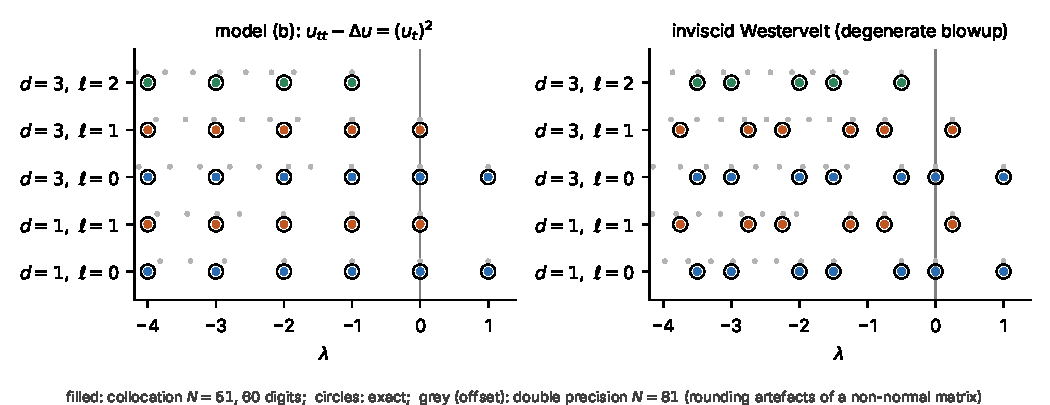
\includegraphics[width=\textwidth]{figures/acou_spectrum.pdf}
\caption{Spectra of the linearisation at the ODE blowup for (RW) (left;
exact: $\lambda=1-j$, $j\ge\ell$) and for the inviscid Westervelt degeneracy
(right; exact: $1-\frac34(\ell+2n)$, $-\frac34(\ell+2n)$). Filled: collocation, $N=61$,
60 digits. Circles: exact. Grey, offset: double precision, $N=81$.}
\label{acou:fig-spec}
\end{figure}

\emph{Tilted blowup in 1D.} We solve (RW) with $u(0)=0$,
$u_t(0)=2/(1+x^2)$ by the characteristic-diamond scheme, which respects the
light cone exactly ($h=10^{-4}$, \texttt{code/acou\_tilt1d.py}). Fitting
$u_t\approx C(x)/(T(x)-t)$ at each $x$ gives a spacelike blowup curve
($\max_{|x|\le1.2}|T'|=0.52$, $T_{\min}=0.5445$). The fitted coefficient
satisfies $|C(x)-(1-T'(x)^2)|\le5\times10^{-4}$, as predicted by
\cref{acou:lem-tilt}. At $x_1=0.8$, with $a=T'(x_1)=0.404$, the rescaled
time derivative $\rho\,u_t(T(x_1)-\rho,x_1+\rho\xi)$ converges to
$(1-a^2)/(1+a\xi)$. The sup-error is $6.1,2.9,1.3,0.64\times10^{-2}$ for
$\rho=0.2,0.1,0.05,0.025$, i.e.\ $O(\rho)$, matching the gap $1$. Its
distance to the ODE profile $1$ stays at $0.41$ (\cref{acou:fig-tilt}).

\begin{figure}[ht]
\centering
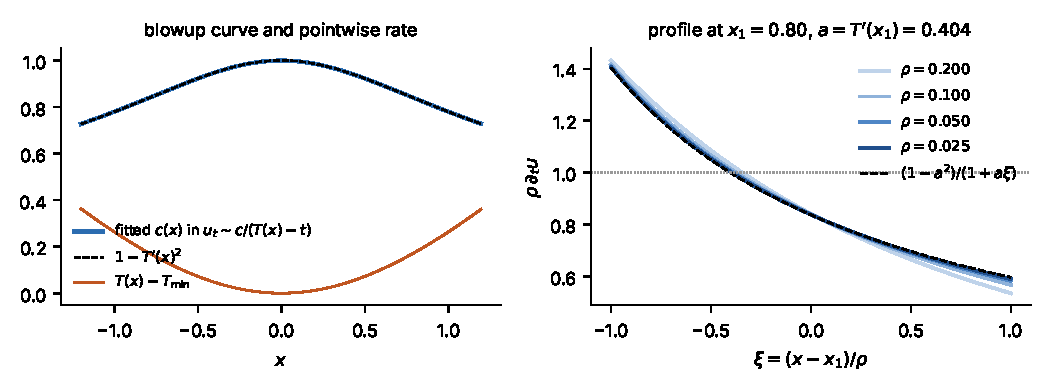
\includegraphics[width=\textwidth]{figures/acou_tilt.pdf}
\caption{(RW) in 1D. Left: blowup curve and pointwise rate coefficient
$C(x)$ versus $1-T'(x)^2$. Right: convergence of $\rho\,\partial_tu$ to the tilted
profile $(1-a^2)/(1+a\xi)$ at a point of the blowup curve with slope $a=0.404$.}
\label{acou:fig-tilt}
\end{figure}

\emph{Westervelt degeneracy in 1D.} We solve \eqref{acou:qeq} ($c=1$, periodic)
with $q(0)=1$, $q_t(0)=-(1+0.2\cos x)$ (\texttt{code/acou\_westervelt1d.py}).
The first degeneracy occurs at $x_0=0$, $T=0.41991$. Fitting
$q^2(t,0)=A\rho+C\rho^{3/2}+D\rho^2+E\rho^{5/2}$ gives $A=2.3092$ and
$C=0.1342$, while the prediction $C=\frac83H/\sqrt A$ with the measured
$H=0.0766$ is $0.1345$, an agreement of $0.2\%$ that is stable under grid
refinement and changes of the fit window. A fit with integer powers only
leaves residuals $2\times10^{4}$ times larger, which confirms the half-integer
expansion predicted by \cref{acou:prop-west}.

\subsection{Summary and caveats}
\label{acou:sub-summary}
\begin{itemize}[nosep]
\item \textbf{(D)} (RW): the linearisation at the ODE blowup is
  \emph{exactly} conjugate to the free wave flow with $s=-1$. Its spectrum
  is $\{1-j\}$, i.e.\ $1-\ell-2n$ and $-\ell-2n$ in the $\ell$-sector, and
  all eigenvalues are semisimple. The neutral $\lambda=0$ modes are the shift
  ($\ell=0$) and the tangents to the exact tilted family $u_{T,a}$
  ($\ell=1$). There is no Jordan block, only a quadratic drift $-|a|^2\tau$
  of $\psi_1$. Radial stability (\cref{acou:thm-rad}) holds with every rate
  $\omega<1$ for $k>\frac d2+2$ (proof sketch).
\item \textbf{(C)} Nonradial stability converges to $u_{T,a}$, not to $u_T$
  (\cref{acou:thm-nonrad}); this is supported by 1D numerics but not proved
  here.
\item \textbf{(K/D)} (NF): explicit via $w=e^{-u}$. The generic first
  blowup is ODE-type with gap $1$ and boosted profiles; non-generic zeros
  give self-similar profiles $-\log P$.
\item \textbf{(D/C)} Westervelt/Kuznetsov ($b=0$): degenerate blowup with
  $p$ bounded and $p_t\sim(T-t)^{-1/2}$, scaling $x\sim(T-t)^{3/4}$, and a
  formal spectrum $\{1-\frac34(\ell+2n)\}\cup\{-\frac34(\ell+2n)\}$. The
  linear structure is Donninger-like, but the nonlinear problem is
  quasilinear and open; it is physically outside the validity of the model.
\item \textbf{(D/C)} The viscous term $b\Delta p_t$ dominates in similarity
  variables, so the light-cone theory does not apply for $b>0$. Heat-type
  blowup is conjectured, but only on picosecond scales.
\item Caveats: semigroup generation on $H^k\times H^{k-1}(B^d)$ for general $d,k$ is
  quoted, not reproved. The nonlinear arguments are sketches. References
  marked \texttt{TODO verify} in the source could not be checked online.
\end{itemize}
